\chapter{NMR Spectroscopy of Proteins}
\begin{center}
  \textit{Nature's imagination far surpasses our own.}

 - Richard Feynman
\end{center}


\section{Physical basis of the NMR experiment}

Some atomic nuclei have non-zero magnetic moments \cite{zeeman1897effect}. 
These can be manipulated using magnetic fields and electromagnetic radiation 
\cite{bloch1946nuclear, rabi1938}.  The discovery was the subject of two 
Nobel prizes, awarded to Rabi in 1944 and to Bloch and Purcell in 1952.

Continuous wave spectroscopy was first employed, in which a frequency source 
was fixed and the magnetic field varied; the absorption was observed and 
collected.  Later, advances led to Fourier Transform spectroscopy, in which
the magnetic field was fixed and all frequencies were collected simultaneously
\cite{aue1976two}.  The Fourier Transform made this possible by allowing the
separation of individual frequency components from the time-domain signal
\cite{ernst2004}.

Nuclei of spin-1/2 are especially well suited to NMR experiments.  In the 
absence of an external magnetic field, spin-1/2 nuclei have two degenerate 
energy levels.  In the presence of an external magnetic field, two distinct 
energy levels are formed as the magnetic moments of the nuclei precess 
around the external magnetic field \cite{hahn1950spin, bloembergen1948relaxation}.

The frequency of the precession is known as the Larmor frequency, and depends 
on the gyromagnetic ratio of the nucleus as well as the strength of the 
magnetic field, which may be modulated due to local effects
\cite{carr1954effects, meiboom1958modified}.

Nearby nuclei can interact through several mechanisms.  Covalently-bonded nuclei
interact through the bonding electrons in a phenomenon known as J-coupling.
Spatially near nuclei interact directly in a phenomenon known as dipole-dipole
coupling.

The phenomenon of chemical shift was discovered when experimental data showed
that nuclei of the same type did not all resonate at the same frequency -- in
fact, their resonance frequencies depended on the local electronic and 
chemical environment \cite{arnold1951variations}.  
It was further discovered that nuclei could interact
with each other, both directly and indirectly.  Direct interactions are 
known as dipole-dipole couplings.  Indirect interactions mediated
by the electrons are known as "scalar couplings".
Multi-dimensional experiments were first proposed by Jean Jeener 
\cite{jeener1979investigation} and later developed by Richard Ernst
\cite{ernst1992nuclear}, for which Ernst later won a Nobel Prize.  
Chemical shifts and nuclear couplings form the basis of modern NMR 
spectroscopy.


\subsection*{Populations}

Spin systems have multiple states with different energies.  The distribution
of spins occupying each energy level are referred to as populations.  Each
energy level may have more or fewer spins than any other energy level.
At equilibrium, the populations are determined by the relative energy levels.  
Spins can move between energy levels, which changes the populations, in a 
process known as a "transition".

Macroscopic effects are observed as longitudinal magnetization
when energy levels are differentially 
populated.  For example, in a uniform static magnetic field, a sample 
containing spin-1/2 nuclei will show a slight variation in the populations of 
the low-energy and high-energy states, according to the Boltzmann distribution.  
This variation is observable at the macroscopic level as a net magnetization in 
the same direction as the external magnetic field.  Different forms of magnetization
may be induced by perturbing the sample.  When the sample is not at equilibrium,
it will gradually relax back to equilibrium by means of a variety of
pathways and transitions.  Some of these pathways and transitions will create
additional macroscopically observable magnetizations.


\subsection*{Transitions}

Transitions allows spins to move from one energy level to another, changing 
the populations.
A transition may move a spin from low energy to high energy or vice versa.
Some transitions involve a change in only one spin, whereas others involve a
change in multiple spins.  Radiofrequency pulses are used to excite transitions
of a single spin.

Fluctuating local magnetic fields also cause transitions.  The frequency of
the fluctuation of the magnetic field determines the energy available, and if 
the energy matches the energy difference of a transition, the fluctuation is 
able to cause relaxation along that transition.  The ability of fluctuating 
magnetic fields to cause such transitions depends on the power available at the 
frequencies matching those of the energy differences (frequencies are directly
proportional to energies), and the distribution of power along the various
frequencies of local magnetic field fluctuation are described by the spectral
density function.


\subsection*{Relaxation}

Relaxation is the process of a spin ensemble in a non-equilibrium state 
returning to an equilibrium state.  As transitions are stimulated,
the populations of energy levels change, decreasing the 
populations of high-energy states decrease and the increasing the populations 
of low-energy ones.

The speed of relaxation depends on the available transitions and their rates.
The spectral density function is related to the molecular weight,
and is the Fourier Transform of the 
correlation function, describing the amount of motion occurring over a 
range of frequencies.  These molecular motions provide a means for relaxation
to occur; thus the significance of the spectral density function is
that it describes the likelihood for relaxation to occur based on resonance
frequencies and energy differences.

In molecules in solution, molecular tumbling causes nuclei to reorient with
respect to the external magnetic field and thus changes the interactions
between coupled nuclei; thus, a nucleus causes its nearby, coupled nuclei to
experience a fluctuating magnetic field and may help them to relax.
Relaxation may be described using the Bloch equations \cite{bloch1946nuclear},
a set of differential equations which describe the change in magnetization 
over time with respect to the difference from the equilibrium state.

There are two separate relaxation rate constants: \mattftone{} describes 
relaxation in the Z or longitudinal axis, parallel to the external magnetic
field.  \mattfttwo{} describes relaxation in the rotating XY plane, also known
as the transverse component.


\subsection*{A spin system of one spin}

In a spin system containing a single nucleus of spin-1/2 \ref{one_spin_1-2},
there are two energy levels, and two transitions between those energy levels
-- one in each direction.  The nucleus' Larmor frequency determines the 
difference between energy levels, which is in turn by determined by the 
local magnetic field, in which electrons play a role.

Since only a single spin's orientation changes when transitioning between
the energy levels, it is termed a "single-quantum transition".
At equilibrium in a static external magnetic field, the difference in 
populations of the two energy levels is governed by the Boltzmann distribution.


\subsection*{Homonuclear AX spin system}

In this spin system \ref{two_spins_1-2}, there are
two nuclear spins of spin-1/2, each of which has two possible spin orientations,
denoted by alpha and beta,
four energy levels, denoted by alpha/alpha, alpha/beta, beta/alpha, and beta/beta, and
twelve transitions between energy levels, grouped into six pairs and denoted
by double-headed arrows.  Associated with each transition is a transition
probability or rate.  These are grouped into three different kinds of transitions:

\begin{itemize} 
  \item zero-quantum.  Both nuclei change their spin orientations, 
     but the energy difference is very small because both in the initial and
     final states, one nucleus is in the high-enery orientation and one is in
     the low-energy orientation

  \item single-quantum.  One nucleus' spin orientation changes, but
     the other does not.  The energy difference is related to the Larmor frequency
     of the nucleus that undergoes the change, meaning that these transitions may
     be exploited in order to capture chemical shifts

  \item double-quantum.  Both nuclei start out with the same spin
     orientation, both spin orientations change, and so both end up with the
     same final spin orientation.  In contrast to the zero-quantum transitions,
     there is a much larger energy difference involved.

\end{itemize}
   
Radio Frequency (RF) pulses are used to induce single-quantum transitions.
Zero- and multiple-quantum transitions are stimulated by fluctuations in 
local magnetic fields.  The alpha/beta and beta/alpha energy levels are 
similar but distinct.  They are both very different from the alpha/alpha 
and beta/beta energy levels.  The spectra of this spin system includes 
two lines, or four lines grouped into pairs if the nuclei are J-coupled.
Sensitivity is determined by the population differences.
In an isotropic medium such as water, dipolar couplings are not observed
because they average out over the population.
However, in an alignment medium, there is incomplete averaging
and so some residual dipolar coupling (RDC) is observed, which indicates 
some information about the relative orientations of the vector connecting
the two nuclei compared to the external magnetic field.


\subsection*{The chemical shift}

The chemical shifts are deviations in the Larmor frequencies of specific 
nuclei based on the local chemical environment, due to varying
electron density.  This is because the electrons can shield or deshield nuclei
from the external magnetic field, modulating the field such that it is weaker
or stronger.

The energy difference between the two spin states is, to a good approximation,
linearly dependent on the local magnetic field strength 
\cite{cavanagh1995protein}.  Therefore, the 
result is that nuclei with different local electron fields which experience
different local magnetic fields will resonate at different frequencies, and
different chemical shifts when those frequencies are normalized with respect
to the strength of the external magnetic field.


\subsection*{The NOE experiment}

The Nuclear Overhauser Effect (NOE) is a relaxation phenomenon in which
longitudinal magnetization is transferred between dipole-dipole coupled spins.
A non-equilibrium population distribution is created using an RF pulse,
which initially affects only one spin, on which
longitudinal magnetization is created.  Initially, the second spin is not
afected.  The spin system then returns to
equilibrium in a process known as relaxation.  Due to the dipole coupling,
there are cross-relaxation pathways available, which transfer longitudinal
magnetization from one nucleus to the other when the appropriate transitions
are stimulated.  The rate at which each transition is utilized depends on the
spectral density function.

The phenomenological equation describing the NOE is 
$ f_I\left\{S\right\} = (I - I_0) / I_0 $.
The strength of the NOE depends on the distance between the nuclei, 
the gyromagnetic ratios, and their orientation relative to the external 
magnetic field, as described by $B(l) = c * m * (3*(cos^2 w)-1) / r^3$
where 
m    is the gyromagnetic ratio,
B(l) is the magnetic field strength due to other nucleus,
w    is the angle between external B field and vector connecting two nuclei, and
r    is the distance between the two nuclei.
The above equation can be expanded using the Solomon equation such that the
% this is all from http://www.bioc.aecom.yu.edu/labs/girvlab/nmr/course/COURSE_2012/RelaxNoe2012.pdf
NOE depends on the $ W_0 $, $ W_1 $, and $ W_2 $ rate constants, giving
$ f_I\left\{S\right\} = c * (W_2 - W_0) / (W_0 + 2 * W_1I + W_2) $.
The equations for the rate constants are as follows:
$ W_0 = K^2 * J * (w_I - w_S) / 20 $,
$ W_1I = 3 * K^2 * J * w_I / 40 $,
$ W_IS = 3 * K^2 * J * w_S / 40 $,
$ W_2 = 3 * K^2 * J * (w_I + w_S) / 10 $,
where I and S refer to the two spins of the two-spin system.

The equilibrium state of the two-spin system in an external magnetic field:
more nuclei are in the low-energy states (for both spins) than in the 
high-energy states \ref{two_spins_initial}.  Application of an RF pulse 
changes the populations of one spin \ref{two_spins_rf}, but does not affect
the other spin.  Cross-relaxation transfers magnetization from one spin to
the other.  If the w0 rate is faster, the high-energy state of the 
second spin will be enhanced \ref{two_spins_w0}.  If the w2 cross-relaxation 
rate is faster, the low-energy state of the second spin will be enhanced 
\ref{two_spins_w2}.



\section{Protein NMR}

Proteins containing spin-1/2 nuclei may be studied using NMR.  Hydrogen, 
Carbon and Nitrogen are all plentiful in proteins, and have isotopes of 
spin-1/2.  Useful biophysical characterization of proteins that may be 
obtained using NMR includes structural, dynamics, and binding information.

\subsection*{Sample preparation}

The first step of an NMR analysis process is to obtain a sample of the protein
of interest.  NMR is a relatively insensitive technique, and so it is important
to get a sample with relatively high concentration compared to other structural
biology techniques, often in the millimolar range.  The protein is produced
by transforming a plasmid into bacteria, and then inducing transcription 
of the plasmid followed by translation.  If specific isotopes, such as 15N or 
13C are required for their NMR properties, they may be provided in the 
bacteria's growth media.  Finally, the protein is isolated and purified
\cite{derome1987modern}.

\subsection*{Data collection}

Assuming the purified, high-concentration protein sample does not aggregate
or denature, NMR experiments are run by placing a tube of the sample inside 
of a spectrometer, running sequences of radio-frequency pulses which selectively
excite nuclei within the sample, and observing the results.  The data a 
superposition of decaying sinusoids of different frequencies and amplitudes;
the frequencies are caused by the precession at the Larmor frequency along with
the resonance phenomenon of the various nuclei, and the decay is the result
of the system gradually relaxing back to equilibrium \cite{bloch1946nuclear}.

Various pulse sequences are used to probe specific functional groups within
the protein.  There are two major categories of pulse sequences, based on the
nature of the interactions they exploit: the first group exploits scalar 
couplings which exist between covalently-bonded nuclei, and are thus called 
"through-bond" experiments \cite{davis1985assignment}.  
The second group exploits dipole-dipole couplings
between protons that are spatially close but do not have to be covalently
bonded, and are thus called "through-space" experiments
\cite{solomon1955relaxation}.  The data produced by
these two experiments are also used in very different ways, as we will see
later.

Two important parameters of data collection are the dwell time and the number
of points collected.  The dwell time determines the range of frequencies that
can be distinguished.  The number of points collected determines the resolution
(the ability to distinguish between nearby, but distinct, frequencies).  Instead
of the number of points, one can also use the acquisition time, which is the
product of the dwell time and the number of points.

Maximizing sensitivity is also helpful for later data analysis.
Sensitivity depends not only on the gyromagnetic ratios of nuclei, but also
on the strength of the external magnetic field due to the magnitude of the
difference between the high- and low-energy states of a spin-1/2 nucleus
according to the Boltzmann distribution.
Running an experiment multiple times and summing the results is a 
means of increasing sensitivity as the signal increases faster
than the noise, assuming random distribution of the noise
\cite{ardenkjaer2003increase}.

Referencing is done to ensure that results are comparable from multiple
spectrometers.  While the absolute Larmor frequencies of nuclei vary depending
on the magnetic field of the spectrometer, the normalized values, when compared
to a known material, of which a small amount is placed in the spectrometer,
are consistent \cite{wishart19951h}.  These are known as chemical shift values,
and are reported in parts per million of deviation.

\subsection*{Spectral processing}

The time-domain experimental data are converted to frequency-domain spectral
data to facilitate analysis.  A decaying sinusoid in the time-domain becomes
a peak with a finite and non-zero linewidth at the corresponding frequency
in the frequency-domain.  The Fourier Transform \cite{cooley1965algorithm}
is a standard method for 
converting between time- and frequency-domains, and is often used on NMR data.
Through appropriate use of scaling and normalization, the frequency axis is
converted to chemical shifts.

The Nyquist theorem \cite{nyquist1928certain, shannon1949communication}
places bounds on the dwell time with respect to the 
final spectral width.  A poor choice of dwell time can lead to spectral 
aliasing, in which peaks appear in unexpected spectral regions because their
frequencies are outside the range supported by the chosen dwell time.
Two factors confound resolution:  coincidental
closeness of resonances frequencies, and experimental quality.  In general, 
larger proteins, which have more atoms than smaller proteins, have more resonance
frequencies in close proximity to each other, increasing the probability of 
overlap.  To increase resolution, it is necessary to collect data points at 
large time intervals.  Care must be taken to avoid decreasing the sensitivity;
non-uniform sampling and Maximum Entropy reconstruction offer one means of so
doing \cite{rovnyak2004accelerated, hoch1985maximum}.

A peak in a through-bond spectrum and in a through-space spectrum have 
different meanings.  In a through-bond spectrum, a peak indicates the 
observation of several resonating nuclei connected by a small number of
covalent bonds.  However, a peak in a through-space NOESY spectrum indicates
the presence of two protons within approximately 5 Angstroms of each other
\cite{neuhaus1989nuclear}.

\subsection*{Peak picking}

Peak picking is the process of identifying signals in an NMR spectrum using
peaks as a proxy.  The position of the multi-dimensional peak indicates the
chemical shifts of the nuclei giving rise to it, and the amplitude may have
significance in some but not all experiments.

Peak picking would be if easy if several conditions were met by the spectra:

\begin{itemize}
  \item all expected signals appear
  \item all signals are easily distinguishable from noise and artifacts
  \item all signals are well dispersed from all others
  \item no unexpected signals appear
\end{itemize}
 
However, in practice, none of these conditions are met \cite{williamson2009automated}.  
Thus, it is commonly
the case that expected signals are missing, some signals are close to the noise
level, some noise appears to be signal, some artifacts appear, signals overlap
to greater or lesser extents, and some unexpected signals appear, perhaps due
to contamination or multiple conformations \cite{baran2004automated}.

Therefore, accurate peak picking must deal with these problems, in order to
identify all the true signals, none of the false signals, and to correctly 
characterize the position and volume of the true signals.  Initial peak picking
is often performed using a computational tool, but there typically is some
level of manual intervention in order to correct mistakes and other problems
\cite{guerry2011automated}.

\subsection*{Chemical shift assignment}

Nuclei in NMR experiments resonate at characteristic frequencies; 
chemical shift assignment is the process of drawing the correspondence between
the resonance frequencies identified from picked peaks and the nuclei in the
protein of interest.  Assignment is typically accomplished using a set of
through-bond spectra, many of which are based around H-N groups and nearby
atoms, and others which obtain the chemical shifts of the aliphatic sidechains
(both carbons and protons) and still others for the aromatic portions of
sidechains \cite{hnco, hncacb, cbcaconh, hbhaconh, cconhtocsy}.

Assignment proceeds through two key intermediate data types: generalized spin
systems (or GSSs) and resonances \cite{bmrb, ccpn}.  
Resonances are the NMR-visible incarnations
of nuclei: they resonate at characteristic frequencies across spectra.  GSSs
are similar to NMR-visible incarnations of amino acid residues, but may span
multiple residues and are therefore networks of covalently-bonded resonances
\cite{abacus_assignment}.

Peaks are assembled into GSSs by exploiting the redundancy between several 
experiments: resonances appear in multiple spectra, at the same characteristic
frequency giving rise to peaks (signals), and this is used to match these
peaks into the same GSSs and resonances.  Peaks can also be matched within
a single spectrum into the same GSS, depending on the nature of the experiment
\cite{ccpn}.

GSSs and resonances can be typed, that is, assigned to an amino acid type or
an atom type respectively.  As can be found in the BMRB, there is large 
variation in average chemical shifts depending on amino acid type and atom type,
especially for Serine/Threonine, Glycine, and Alanine residues, for which the
CB, CA, and CB atoms' chemical shifts are essentially unique
\cite{guntert2009automated}.

A second type of overlap is used in chemical shift assignment: due to the 
similar J-couplings of the CA both of the previous and same residue to the
backbone Nitrogen, it is possible to correlate a backbone amide group with
both adjacent sidechains.  Thus, each sidechain may be correlated with two
backbone amide groups, causing their resonances to appear in conjunction with
two other groups.  As the atoms resonate at a characteristic frequency, this
can be used to identify a sequential connection between the two GSSs based on
backbone amide groups.  Once a sufficiently long chain is built using these
sequential connections and the (possibly incomplete) GSS typings, the chains 
may be assigned to specific residues in the protein sequence.  Combined with
resonance typing, this is sufficient to obtain chemical shift assignments
\cite{hnco, hncacb, cbcaconh}.

However, chemical shift assignment is complicated by missing, overlapped, and
extraneous signals, as well as ambiguities in GSS typings, resonance typings,
sequential GSS connectivity, and sequence-specific GSS-residue assignments
\cite{williamson2009automated, guerry2011automated}.
The ambiguities in typings are caused by the non-uniqueness of average chemical
shifts for most residue types (apart from Glycine, Alanine, Serine, and 
Threonine) \cite{bmrb}.  The ambiguities in sequential
assignments are caused by degenerate chemical shifts across multiple residues,
as well as by missing and extraneous signals, and those in sequence-specific
assignments are caused by non-uniqueness of the match between GSS typing
of a sequential chain and the primary sequence of the protein.

Accurate and complete chemical shift assignment requires nearly complete and
correct peak picking, as well as the presence in the spectra of nearly complete
expected signals, well-dispersed such that there is little to no overlap
\cite{guntert2009automated, guerry2011automated}.
It is often helpful to use a computational tool to quickly assign most of the
chemical shifts, but later to make manual interventions to fix mistakes and
assign any missed resonances \cite{baran2004automated}.

\subsection*{NOESY assignment}

NOESY spectra provide distance restraints between proton pairs.  In order to
make use of their latent structural information, the peaks must be assigned
to resonances and thereby to atoms.  This is done with the help of the 
chemical shift assignments: NOESY peak cross-sections are matched to atoms
based on similarity of the cross-section's chemical shift to that of the
resonance assigned to the atom.

However, NOESY data are heavily ambiguous, because there are typically several
resonances with chemical shift values close enough to match a single NOESY
peak cross-section.  There are several strategies for mitigating this problem.
One is to collect 3D or 4D NOESY experiments, in which the additional dimensions
correlate covalently-bonded 13C or 15N nuclei to the protons involved in the
NOE interaction \cite{majumdar1993improved}.  
This approach greatly reduces the ambiguity.  Furthermore,
characteristic peak patterns are expected, such as intra-residue NOESYs between
protons of that residue, as well as NOESY peaks between protons of sequential
residues.  Another approach is selective labeling \cite{takeda2007automated}.

Accurate and complete NOESY interpretation requires nearly complete chemical
shift assignment.  Furthermore, some manual intervention in NOESY assignment
may be necessary to correct and validate troublesome cases, or to prevent
automated assignment programs from making mistakes 
\cite{guntert2009automated, guerry2011automated}.

NOESY data may be assigned manually, but are often assigned computationally
as well, or with a combination of the approaches.  The CYANA and ARIA structure 
calculation programs include facilities for automated NOESY assignment
\cite{cyana2004, aria2003}.  
A third tactic for dealing with ambiguous NOESY data is to iteratively reduce the
ambiguity using network-anchoring approaches, that use initial structure 
estimates to drive further unambiguous NOESY assignment in a self-consistent
cycle \cite{cyana2004, aria2003}.

\subsection*{Structure calculation}

There are several other types of structural information obtained through NMR
besides the proton-proton distance restraints provided by NOESY spectra.
Using a program such as TALOS+ \cite{talos+}, backbone torsion angles can be 
predicted.  TALOS+
uses the chemical shift assignments of backbone atoms in conjunction with a
database search to make its predictions.  3-J-coupling constants can be 
related to dihedral torsion angles through the Karplus equation
\cite{karplus1959contact, karplus1963vicinal}.  Residual dipolar couplings
(RDCs) provide information about bond orientations.

These data are synthesized into a structural model by programs including CYANA,
ARIA, and XPLOR-NIH.  CYANA is useful for quickly obtaining coarse structure
estimates.  XPLOR-NIH is able to provide more detailed structural models, but
may take far longer to calculate a structure \cite{xplor-nih, cyana2004}.

\subsection*{Deposition}

The BMRB is the main repository for information derived using NMR spectroscopy.
A BMRB deposition may be prepared that includes chemical shift assignments,
peaks, peak assignments, binary spectral and time-domain data, sample 
preparation protocol, and various other relevant data.  The PDB is the main 
repository for structural data.  It is possible and useful to link a BMRB
deposition to a PDB deposition \cite{bmrb, pdb}.




% figures
\clearpage
\section{Figures}

\begin{figure}[h]
  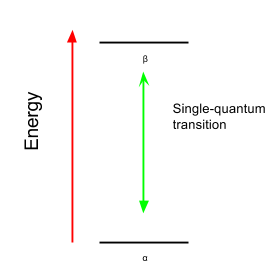
\includegraphics[scale=0.5]{figures/one_spin_1-2}
  \caption{An energy-level diagram for a spin system of a single nucleus.}
  \label{one_spin_1-2}
\end{figure}

\begin{figure}[h]
  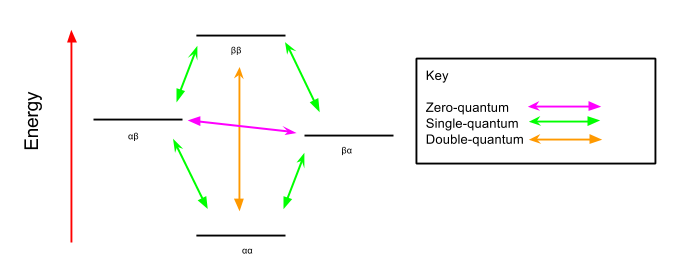
\includegraphics[scale=0.5]{figures/two_spins_1-2}
  \caption{An energy-level diagram for a spin system containing two nuclei.}
  \label{two_spins_1-2}
\end{figure}

\begin{figure}[h]
  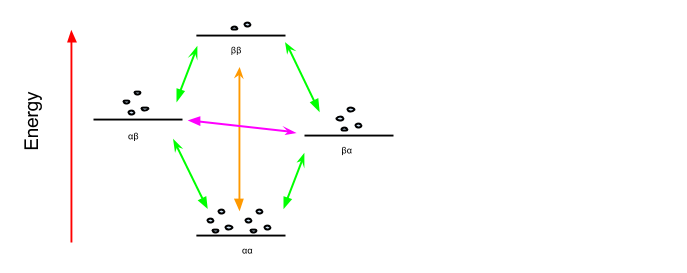
\includegraphics[scale=0.5]{figures/two_spins_initial}
  \caption[The initial population distribution of a two-spin system.]
          {The initial population distribution of a two-spin system in a 
           static uniform magnetic field.  The low-energy states of both
           spins are more populated than the high-energy states, according to
           the Boltzmann distribution.}
  \label{two_spins_initial}
\end{figure}

\begin{figure}[h]
  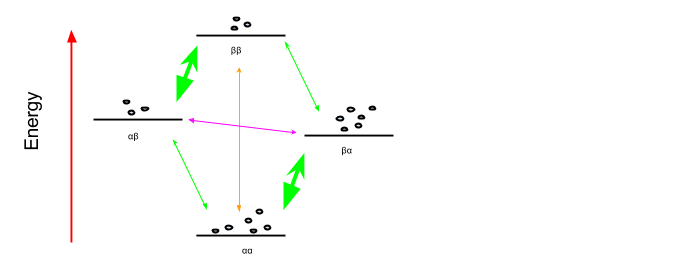
\includegraphics[scale=0.5]{figures/two_spins_rf}
  \caption[An RF pulse on one nucleus equalizes its populations.]
          {An RF pulse on one nucleus equalizes its populations, in a 
           single-quantum transition.  The population of the second spin
           is unchanged.}
  \label{two_spins_rf}
\end{figure}

\begin{figure}[h]
  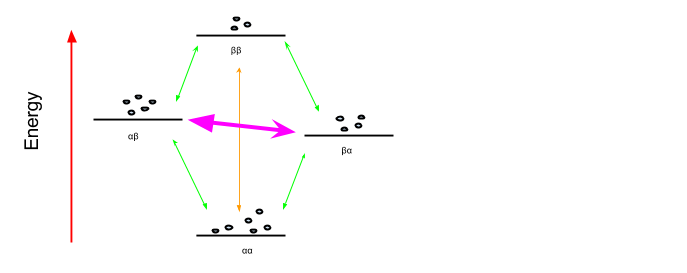
\includegraphics[scale=0.5]{figures/two_spins_w0}
  \caption[Cross-relaxation along the zero-quantum transition.]
          {Cross-relaxation along the zero-quantum transition leads to 
           an increase in the high-energy population of the second spin.}
  \label{two_spins_w0}
\end{figure}

\begin{figure}[h]
  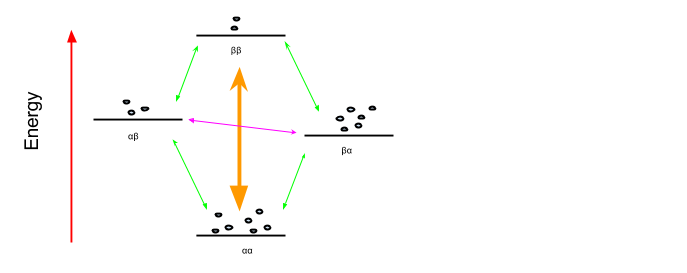
\includegraphics[scale=0.5]{figures/two_spins_w2}
  \caption[Cross-relaxation along the double-quantum transition.]
          {Cross-relaxation along the double-quantum transition leads to
           a decrease in the high-energy population of the second spin.}
  \label{two_spins_w2}
\end{figure}

